\section{Derivation of Stiffness Matrix}
\begin{figure}
	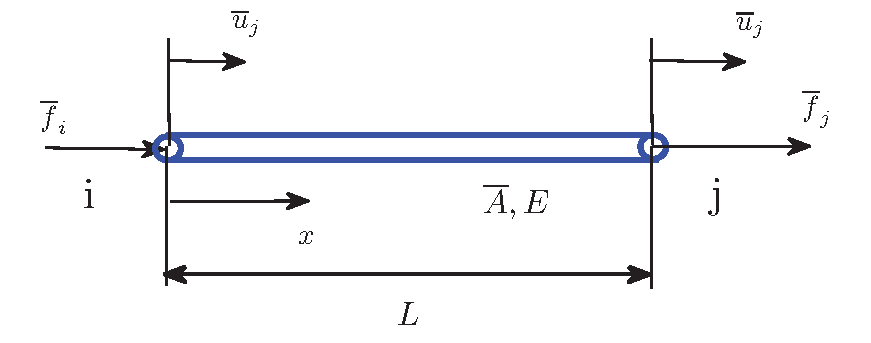
\includegraphics[width=\textwidth]{../figures/a-typical-element}
	\caption{A Typical Bar Element}
	\label{fig:A_Typical_Element}
\end{figure}
Imagine a uniform prismatic bar of length \gls{L}, cross-sectional area $\overline{A}$ and modulus of elasticity $E$. The bar is
elongated \gls{Delta} under an axial uniform force \gls{F}, see \cref{fig:A_Typical_Element}. This is obviously simplified version
of \cref{prb:Non_Normalized_Problem} as both \glssymbol{q} and \glssymbol{f} are constant. In this section we apply first FEM to
derive stiffens matrix for this problem. Then we look at two alternative approaches.
%
\subsection{Using Linear Basis-Functions}
Let us now derive the stiffness matrix of this problem with linear-FEM. From \cref{eqn:Dim_Less_q} we have
\begin{equation}
	q = \frac{ \overline{q} \left( Lx \right) }{ \overline{q} \left( 0 \right) }
		= \frac{ E \overline{A} \left( Lx \right) }{ E \overline{A} \left( 0 \right) }
		= \frac{ \overline{A} \left( Lx \right) }{ \overline{A} \left( 0 \right) } = 1.
\end{equation}
The last equality comes from the fact that the bar's cross-sectional area is uniform, i.e., the area change under the axial load
is negligible. Next we calculate entries of the stiffness matrix. Now set number of elements to
$N = 1$, which also gives $h = 1$. Then the global stiffness and single element matrices are identical, given by
\cref{eqn:Element_Stiffness_Entries_3}. Thus for $i, j = 1, 2$ we have 
\begin{equation}	\label{eqn:Stiffness_Matrix_FEM_Linear_1}
	\begin{aligned}
		\glsentryname{Kij} &= \frac{1}{h} \int_{0}^{1} q \Bigl[ \left( e - 1 + \xi \right) h \Bigr]
		\frac{ d \psi_i }{ d \xi } \frac{ d \psi_j }{ d \xi } \dd \xi	\\
		&= \int_{0}^{1} \frac{ d \psi_i }{ d \xi } \frac{ d \psi_j }{ d \xi } \dd \xi.
	\end{aligned}
\end{equation}
Then the normalized counterpart of the stiffness matrix in \cref{eqn:Stiffness_Matrix_Direct,eqn:Stiffness_Matrix_Formal} follows
after inserting for derivatives of linear basis functions, $\psi_1^{\prime} \left( \xi \right) = -1$ and
$\psi_2^{\prime} \left( \xi \right) = 1$,
\begin{equation}	\label{eqn:Stiffness_Matrix_FEM_Linear}
	\mathbf{K} = \begin{bmatrix}
		1	& -1	\\
		-1	& 1.
	\end{bmatrix}
\end{equation}
%
\subsection{A Direct Approach}
Stiffness matrix in \cref{eqn:Stiffness_Matrix_FEM_Linear} may also be derived by other approaches. In the following we introduce
two such methods, a direct and a formal approach.	\\	\\
Now assume a linear variation of \gls{uBar} above along the bar axis. Thus
\begin{equation}	\label{eqn:Disp_Direct}
	\gls{u} = \left[ 1 - \frac{z}{L} \right] \overline{u}_i + \frac{z}{L} \overline{u}_j.
\end{equation}
The strain \gls{epsilon} along the element is
\begin{equation}	\label{eqn:Strain_Prismatic_Bar_1}
	\gls{epsilon} = \frac{ d \overline{u} }{ dz } = \frac{ \overline{u}_j - \overline{u}_i }{ \gls{Delta} } =
	\frac{ \gls{Delta} }{ L }.
\end{equation}
Next we consider the stress $\sigma$ in the bar
\begin{subequations}
	\begin{align}
		\gls{sigma} &= \frac{ \gls{F} }{ \overline{A} },	\label{eqn:Stress_General}	\\
		\gls{sigma} &= E \gls{epsilon} = \frac{ E \gls{Delta} }{ L }.	\label{eqn:Stress_Prismatic_Bar}
	\end{align}
\end{subequations}
Combining \cref{eqn:Stress_General,eqn:Stress_Prismatic_Bar} results in
\begin{subequations}
	\begin{align}
		\gls{F} &= \glssymbol{KBar} \gls{Delta},	\label{eqn:Bar_Force}	\\
		\glssymbol{KBar} &= \frac{E \overline{A}}{ L }.	\label{eqn:Bar_Stiffness}
	\end{align}
\end{subequations}
The quantity \glssymbol{KBar} in \cref{eqn:Bar_Stiffness} is called the \gls{KBar}. In this case the bar is acting like a spring
with stiffness \glssymbol{KBar}. Thus
\begin{equation}	\label{eqn:Stiffness_Matrix_Direct}
	\gls{matKBar} =
	\begin{bmatrix}
		\glssymbol{KBar}	&		-\glssymbol{KBar}	\\
		-\glssymbol{KBar}	&		 \glssymbol{KBar}
	\end{bmatrix} = \glssymbol{KBar}
	\begin{bmatrix}
		1		&		-1	\\
		-1	&		 1
	\end{bmatrix}.
\end{equation}
\begin{remark}
	\cref{eqn:Stiffness_Matrix_Direct} can be verified by considering equilibrium equation, i.e.,
	\begin{equation}	\label{eqn:Stiffness_Matrix_Direct_Verify}
		\glssymbol{KBar}
		\begin{bmatrix}
			1		&		-1	\\
			-1	&		 1
		\end{bmatrix}
		\begin{bmatrix}
			\overline{u}_i \\
			\overline{u}_j
		\end{bmatrix} =
		\begin{bmatrix}
			\overline{f}_i \\
			\overline{f}_j
		\end{bmatrix}.
	\end{equation}
\end{remark}
\begin{remark}
	The element stiffness matrix in \cref{eqn:Stiffness_Matrix_Direct} has a physical meaning: The $j$-th
	column\footnote{Here $j = 1, 2$.} of \gls{matKBar} represents the necessary forces in the bar to maintain a deformed shape
	with zero and unit displacements at the ends of the bar, nodes $i$ and $j$ respectively.
\end{remark}
%
\subsection{A Formal Approach}
We could also derive element stiffness matrix in \cref{eqn:Stiffness_Matrix_FEM_Linear} using a formal approach. This approach is
more general and may be applied to many other and more complicated situations. \\	\\
Define a vector for nodal shape functions
\begin{subequations}
	\begin{align}
		\gls{psiVec} &= \gls{psiVec} \left( x \right) =
		\begin{bmatrix} \psi_i \left( x \right)	& \psi_j \left( x \right) \end{bmatrix},	\\
		\psi_i \left( x \right) &= 1 - x,	\label{eqn:Shape_Func_Ni}	\\
		\psi_j \left( x \right) &= x,		\label{eqn:Shape_Func_Nj}	\\
	\end{align}
	where
	\begin{equation}
		x = \frac{z}{L},	\quad	0 \leq x \leq 1.
	\end{equation}
\end{subequations}
From \cref{eqn:Disp_Direct} displacement of the bar may then be written as
\begin{equation}	\label{eqn:Disp_Formal}
	\gls{u} = \gls{uBar} = \psi_i \left( x \right) \overline{u}_i + \psi_j \left( x \right) \overline{u}_j =
	\gls{psiVec} \gls{vecuBar}.
\end{equation}
Differentiating \cref{eqn:Disp_Formal} gives strain in the bar
\begin{subequations}
	\begin{align}
		\epsilon &= \frac{ d \overline{u} }{ dz } = \frac{ d }{ dz } \Bigl[ \gls{psiVec} \gls{vecuBar} \Bigr]
			= \frac{ d \gls{psiVec} }{ dz } \gls{vecuBar} = \gls{eVec} \gls{vecuBar}	\label{eqn:Strain_Formal} \\
		\gls{eVec} &= \frac{ d \gls{psiVec} }{ dz }	= \frac{ d \gls{psiVec} }{ dx } \frac{ dx }{ dz }
			= \begin{bmatrix} -1/L & 1/L \end{bmatrix}, \label{eqn:Strain_Disp_Vector}
	\end{align}
\end{subequations}
where \gls{eVec} is the element strain-displacement matrix. Stress in the bar is
\begin{equation}	\label{eqn:Stress_Formal}
	\gls{sigma} = E \gls{epsilon} = E \gls{eVec} \gls{vecuBar}.
\end{equation}
Next consider the strain energy stored in the bar and apply \cref{eqn:Stress_Formal,eqn:Strain_Formal}
\begin{equation}	\label{eqn:Strain_Energy}
	\begin{aligned}
		\gls{U} &= \frac{1}{2} \int_V \sigma^T \epsilon \dd V
			= \frac{1}{2} \int_V \bigl( \gls{vecuBar}^T \gls{eVec}^T E \gls{eVec} \gls{vecuBar} \bigr) \dd V	\\
		&= \frac{1}{2} \gls{vecuBar}^T \Biggl[ \int_V \bigl( \gls{eVec}^T E \gls{eVec} \bigr) \dd V \Biggr] \gls{vecuBar}.
	\end{aligned}
\end{equation}
The total amount of work done by the two nodal forces is
\begin{equation}	\label{eqn:Work_Formal}
	\gls{W} = \frac{1}{2} \overline{f}_i \overline{u}_i + \frac{1}{2} \overline{f}_j \overline{u}_j =
	\frac{1}{2} \gls{vecuBar}^T \gls{vecfBar}.
\end{equation}
Law of \gls{energyConservation} states that in an isolated system the energy can neither be created nor destroyed. Thus
a work amount done on the bar\footnote{By an external force} will not vanish, but increases the system's strain energy, i.e.,
\begin{equation}	\label{eqn:Energy_Cons}
	\gls{W} = \gls{U}.
\end{equation}
Combining \cref{eqn:Energy_Cons,eqn:Work_Formal,eqn:Strain_Energy} we get
\begin{equation}
	\begin{aligned}
		\frac{1}{2} \gls{vecuBar}^T \Biggl[ \int_V \bigl( \gls{eVec}^T E \gls{eVec} \bigr) \dd V \Biggr] \gls{vecuBar}
			&= \frac{1}{2} \gls{vecuBar}^T \gls{vecuBar},	\\
		\Biggl[ \int_V \bigl( \gls{eVec}^T E \gls{eVec} \bigr) \dd V \Biggr] \gls{vecuBar} &= \gls{vecfBar}.
	\end{aligned}
\end{equation}
Thus
\begin{subequations}
	\begin{align}
		\gls{matKBar} \gls{vecuBar} &= \gls{vecfBar},
		\intertext{where}
		\gls{matKBar} &= \int_V \bigl( \gls{eVec}^T E \gls{eVec} \bigr) \dd V.	\label{eqn:Stiffness_Matrix_Formal_1}
	\end{align}
\end{subequations}
%
\begin{remark}
	Element stiffness matrix in \cref{eqn:Stiffness_Matrix_Formal_1} is a general result which can be used for the construction of other types of elements. This result may also be derived using other more rigorous approaches, such as the principle of \gls{minPotentialEnergy} or the \gls{GalerkinMethod}.
\end{remark}
Now, we may evaluate \cref{eqn:Stiffness_Matrix_Formal_1} for the bar element by using \cref{eqn:Strain_Disp_Vector}
\begin{equation}	\label{eqn:Stiffness_Matrix_Formal} 
	\begin{aligned}
		\gls{matKBar} &= \int_0^L
		\begin{bmatrix} -1/L \\ 1/L \end{bmatrix} E 
			\begin{bmatrix} 1/L	& 1/L \end{bmatrix} \overline{A} \dd z \\
		&= \frac{ E \overline{A} }{ L } \begin{bmatrix} 1 & -1	\\ -1 &	1 \end{bmatrix},
	\end{aligned}
\end{equation}
%
which is the same result as \cref{eqn:Stiffness_Matrix_Direct}, direct method. Finally, combining
\cref{eqn:Stiffness_Matrix_Formal,eqn:Strain_Energy}, the strain energy stored in the bar may be written as
\begin{equation}
	U = \frac{1}{2} \left. \gls{vecuBar} \right.^T \gls{matKBar} \gls{vecuBar}.
\end{equation}
%